\section{The signals}
\label{sec:signal}

We search for several models of heavy resonances decaying to
a W or Z boson on one side, and a Higgs on the other, in which both bosons 
decay to quarks producing merged jet.  This analysis is focused on two
channels:
\begin{itemize}
\item \HbbVqq, and
\item \HwwVqq
\end{itemize}
As previously discussed, we use one V-tagging and two Higgs tagging algorithms
to identify such events.  After subdividing the events according to 
high purity and low purity tags, we end up with five distinct categories,
as shown in Table~\ref{table:categories}.

In this section, we discuss various issues related to the evaluation
of the signal efficiency.

% For Higgs decays to \bbbar, we use a pruned jet mass and also b
% tagging to discriminate higgs jet from QCD jets and jets from the
% fully merged hadronically decaying top quark.
% Fig.~\ref{fig:JetMassTagging} shows the pruned jet mass distribution for
% Higgs jet, $\Zqq$ jet, hadronic top jets and QCD jets.



\subsection{Cross-talk between the Higgs decay channels}
\label{sec:cross-talk}

In order to combine events from all categories into a single joint
likelihood, the categories must be mutually exclusive. However, a
cross-talk between the Higgs channels is nevertheless possible: for
example, $\Hbb$ tagger can identify other two-prong Higgs decay modes
like ${\rm H\to gg}$, $H \to \tau \tau$, or ${\rm H \to c\bar{c}}$,
although this kind of `false positive' tag happens only rarely (the
efficiency is $\lesssim 7~\%$).  Similarly, events from two-prong
Higgs decay channels can also pass the $\tau_{42}$ cut in the
$\Hww$ selection.  In this case, the channel $\Hbb$, because of its large
branching ratio, contributes a non-negligible number of events to the
sample of 4q tags.  This effect is illustrated by
Fig.~\ref{fig:HiggsTau42}, where it can be seen that most of the
low-$\tau_{42}$ tail of the $\Hbb$ curve will be below the cut value of 0.55.
\begin{figure}[htb]
\centering
\begin{tabular}{cc}
%     \resizebox{0.5\linewidth}{!}{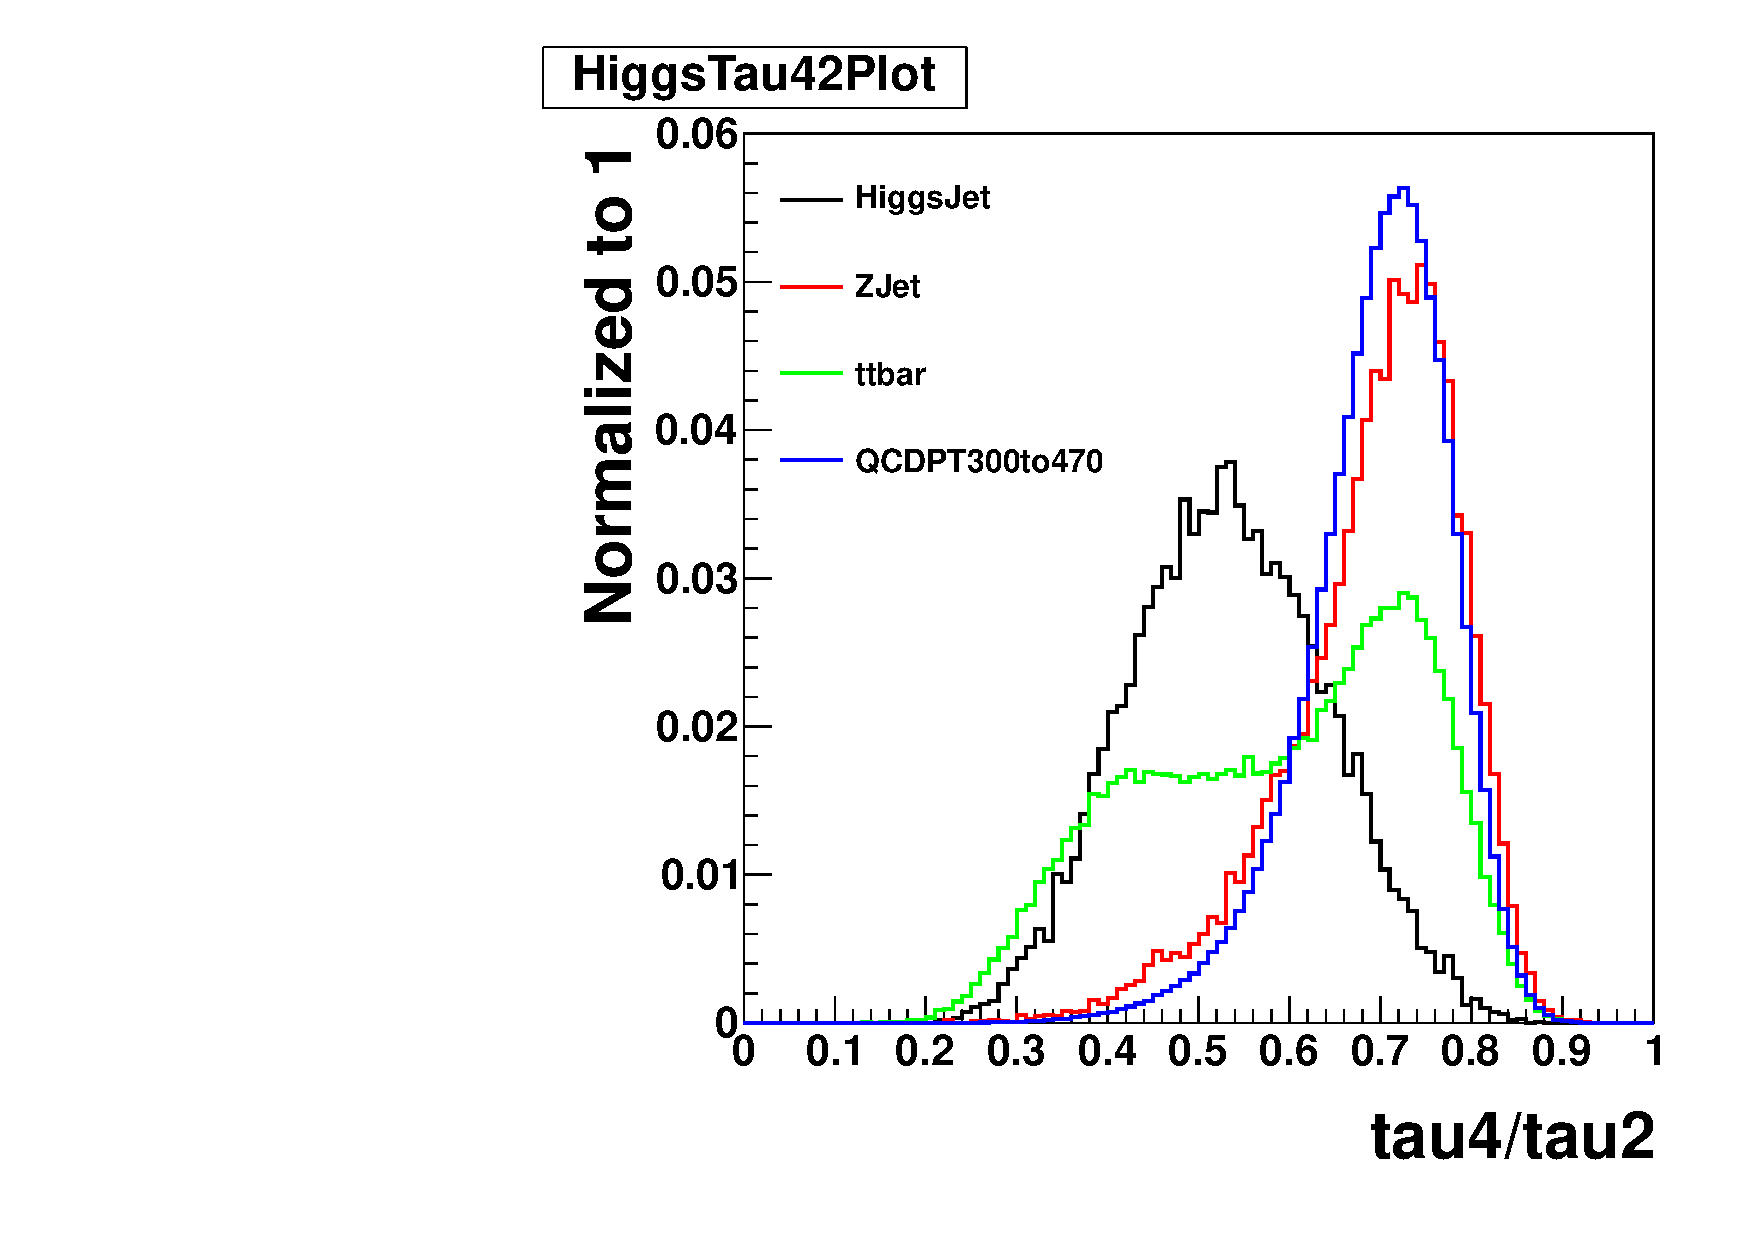
\includegraphics{HqqqqZqqfigs/N-subjettiness/Tau421TeVPre.pdf}} &
     \resizebox{0.7\linewidth}{!}{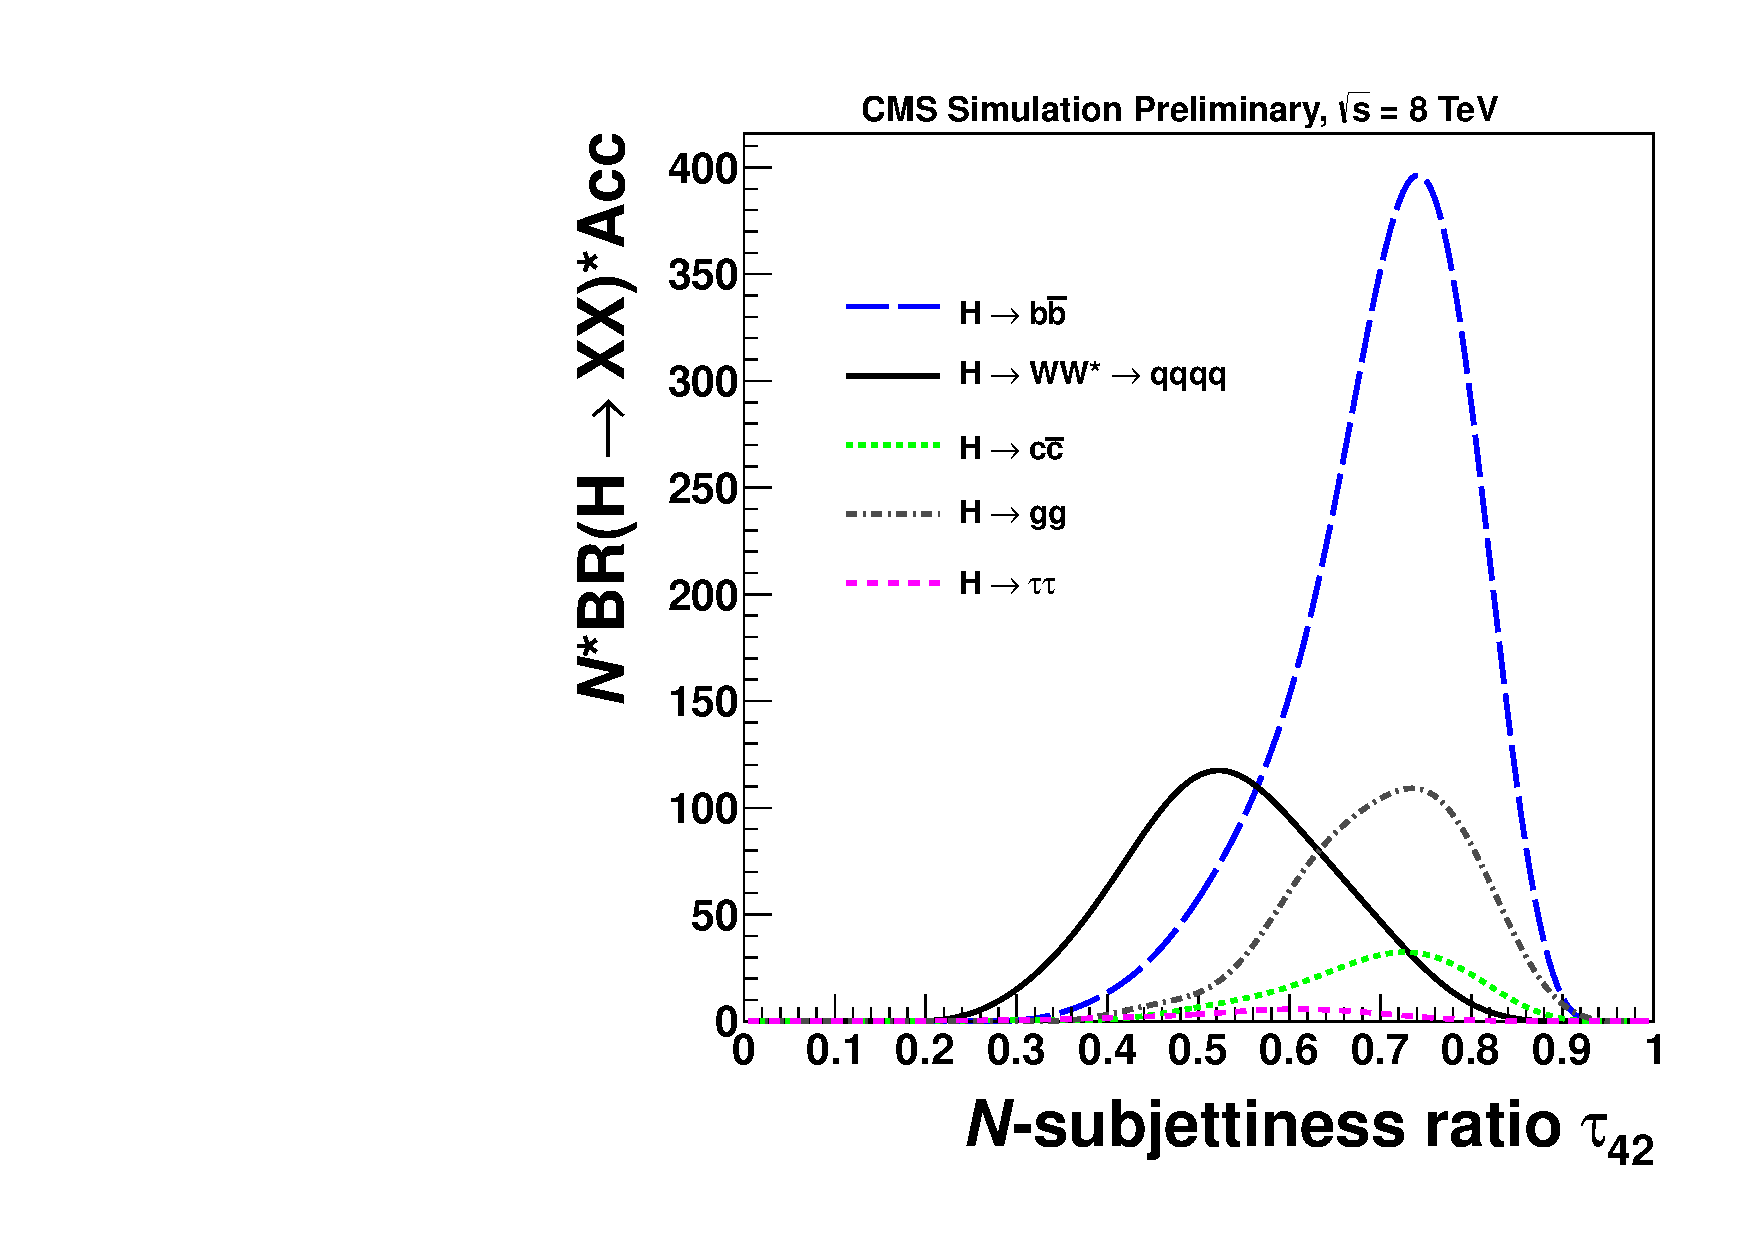
\includegraphics{EXO-14-009/HqqqqZqqfigs/cross-talk/cross-talk.pdf}} \\
\end{tabular}
\caption{Comparison of $\tau_{42}$ distributions 
for signal events failing the $\Hbb$ requirement. 
These events are from the $\Hww$, $\Hbb$, ${\rm H\to gg}$, 
${\rm H \to c\bar{c}}$, and ${\rm H \to} \tau \tau$ channels.
The H jets are from a 1.5~TeV resonance decaying to VH.
%The H jets are from HV signals with a 1.5~TeV resonance.
All curves are normalized to the product of the corresponding branching
fraction and acceptance.}
\label{fig:HiggsTau42}
\end{figure}
 

%\newpage
%\section{Hbb HWW and other Channels}
%\label{sec:contamination}

Table~\ref{table:HbbHww} provides an overview of the cross-talk
between the various channels.  The Higgs branching ratios correspond
to the Higgs mass of 125\GeVcc. 
 For ${\rm H \to WW^* \to 4q }$,
the branching ratio of the hadronic decay of (real) W boson is already 
included, so that the final state is four quarks.
%
The table is normalized to 100,000 standard model Higgs
bosons, and the numbers in the
table show the number of Higgs decays that pass the tagger for each
channel, with the branching ratio taken into account.  
For example, 
let us consider ${\rm H \to c\bar{c}}$ channel.  At the ${\rm Z'}$ resonance
mass of 1.5~TeV, out of 100,000$\times$3.0\% ${\rm H \to c\bar{c}}$ decays,  121 of them
are tagged by the $\Hbb$ tagger  
and  88 of them pass $\Hww$ tagger but fail $\Hbb$ tagger.
For ${\rm H \to ZZ}$ decays, we take its tagging efficiency the same 
as $\Hww$ signals. So the number of ${\rm H \to ZZ}$ to pass $\Hbb$ and 
$\Hww$ tagger is estimated by 
efficiency of $\Hww$ signal times 
 $\mathcal{B}$($H \to ZZ$)$\times \mathcal{B}$($Z \to qq$)$\times\mathcal{B}$($Z\to qq$) divided by 
 $\mathcal{B}$($H \to WW$)$\times\mathcal{B}$($W \to qq$)$\times\mathcal{B}$($W\to qq$). 

%From Table~\ref{table:HbbHww}, it can be seen that for various signal 
%resonance masses, the contribution of other decay channels compared to the 
%sample of $\Hbb$ tags never exceeds 6\%. 

%of the systematic uncertainties, and we do not correct for it.

%And also the ratio of other signals, i.e. Htt, Hgg, Hcc to pass $\Hww$
%tagger, is around 14\% of $\Hww$ plus $\Hbb$ decay modes.
%Their contamination in data should be very tiny.  

Since the $\Hbb$ tagger has significantly lower background than $\Hww$,
it takes precedence in selecting events: we first identify the
events that pass the $\Hbb$ tagger, and only if they fail,  we
test them for the presence of the $\Hww$ tag.  



The effect of the $\Hbb$ tagger veto on the $\Hww$ tagged dijet 
mass distribution
background (data) is shown in Appendix~\ref{appendix:crosstalkData}.
%The fraction of $\Hww$ tags which are also $\Hbb$ tags are small,
%about 3\%, and it is roughly a slowly
% rising slope as a function of the dijet
%invariant mass.


\begin{table}[htbp]
\begin{center}
\caption{Number of Higgs jets falls into two exclusive categories, assuming we have 100,000 SM Higgs (125 GeV) decays to all channels.}
%$\Hzz$ signals are estimated by its branching ratio times the efficiency of $\Hww$ signals divided by the branching ratio of $\Hww$ channel.
\begin{tabular}{cccc}
\hline
%& \multicolumn{1}{l|}{Branching ratio (\%)} & \multicolumn{1}{l|}{Pass $\Hbb$} & \multicolumn{1}{l|}{Pass $\Hww$} & \multicolumn{2}{l|}{Fail $\Hbb$, pass $\Hww$} \\ \hline
& Branching  & Pass       & Fail $\Hbb$, pass \\
& ratio (\%) & $\Hbb$  &   $\Hww$ \\ 
\hline
1.5 TeV  & & & \\
$\Hbb$ & 57.70 & 11444 &  755 \\ %\hline
$\Hww$ & 9.94 & 228 & 1916 \\ % \hline
$\Hzz$ & 1.30 & 29 & 250 \\ % \hline
${\rm H\to c\bar{c}}$ & 3.00 & 121 & 88 \\ %\hline
${\rm H\to} \tau \tau$ & 6.30 & 12  & 57 \\ %\hline
${\rm H\to gg}$ & 10.00 & 69 & 174 \\ %\hline
% & \multicolumn{1}{l|}{} & \multicolumn{1}{l|}{} & \multicolumn{1}{l|}{} & \multicolumn{1}{l|}{} \\
\hline
\\
2.0 TeV &  & & \\ %\multicolumn{1}{l|}{Braching Ratio (\%)} & \multicolumn{1}{l|}{Pass $Hbb$ tagger} & \multicolumn{1}{l|}{Pass Hww tagger} & \multicolumn{1}{l|}{Fail $Hbb$, pass Hww} \\ \hline
$\Hbb$ & 57.70 & 13816 & 551 \\ %\hline
$\Hww$ & 9.94 & 449 & 1435 \\ %\hline
$\Hzz$ & 1.30 & 58 & 187 \\ %\hline
${\rm H\to c\bar{c}}$ & 3.00 & 228 & 99 \\ %\hline
${\rm H\to} \tau \tau$ & 6.30 & 42 & 74 \\ %\hline
${\rm H\to gg}$ & 10.00 & 157  & 262 \\ \hline
\end{tabular}
\label{table:HbbHww}
\end{center}
\end{table}






%\begin{figure}[htb]
%\begin{figure}[ht]
%\begin{center}
%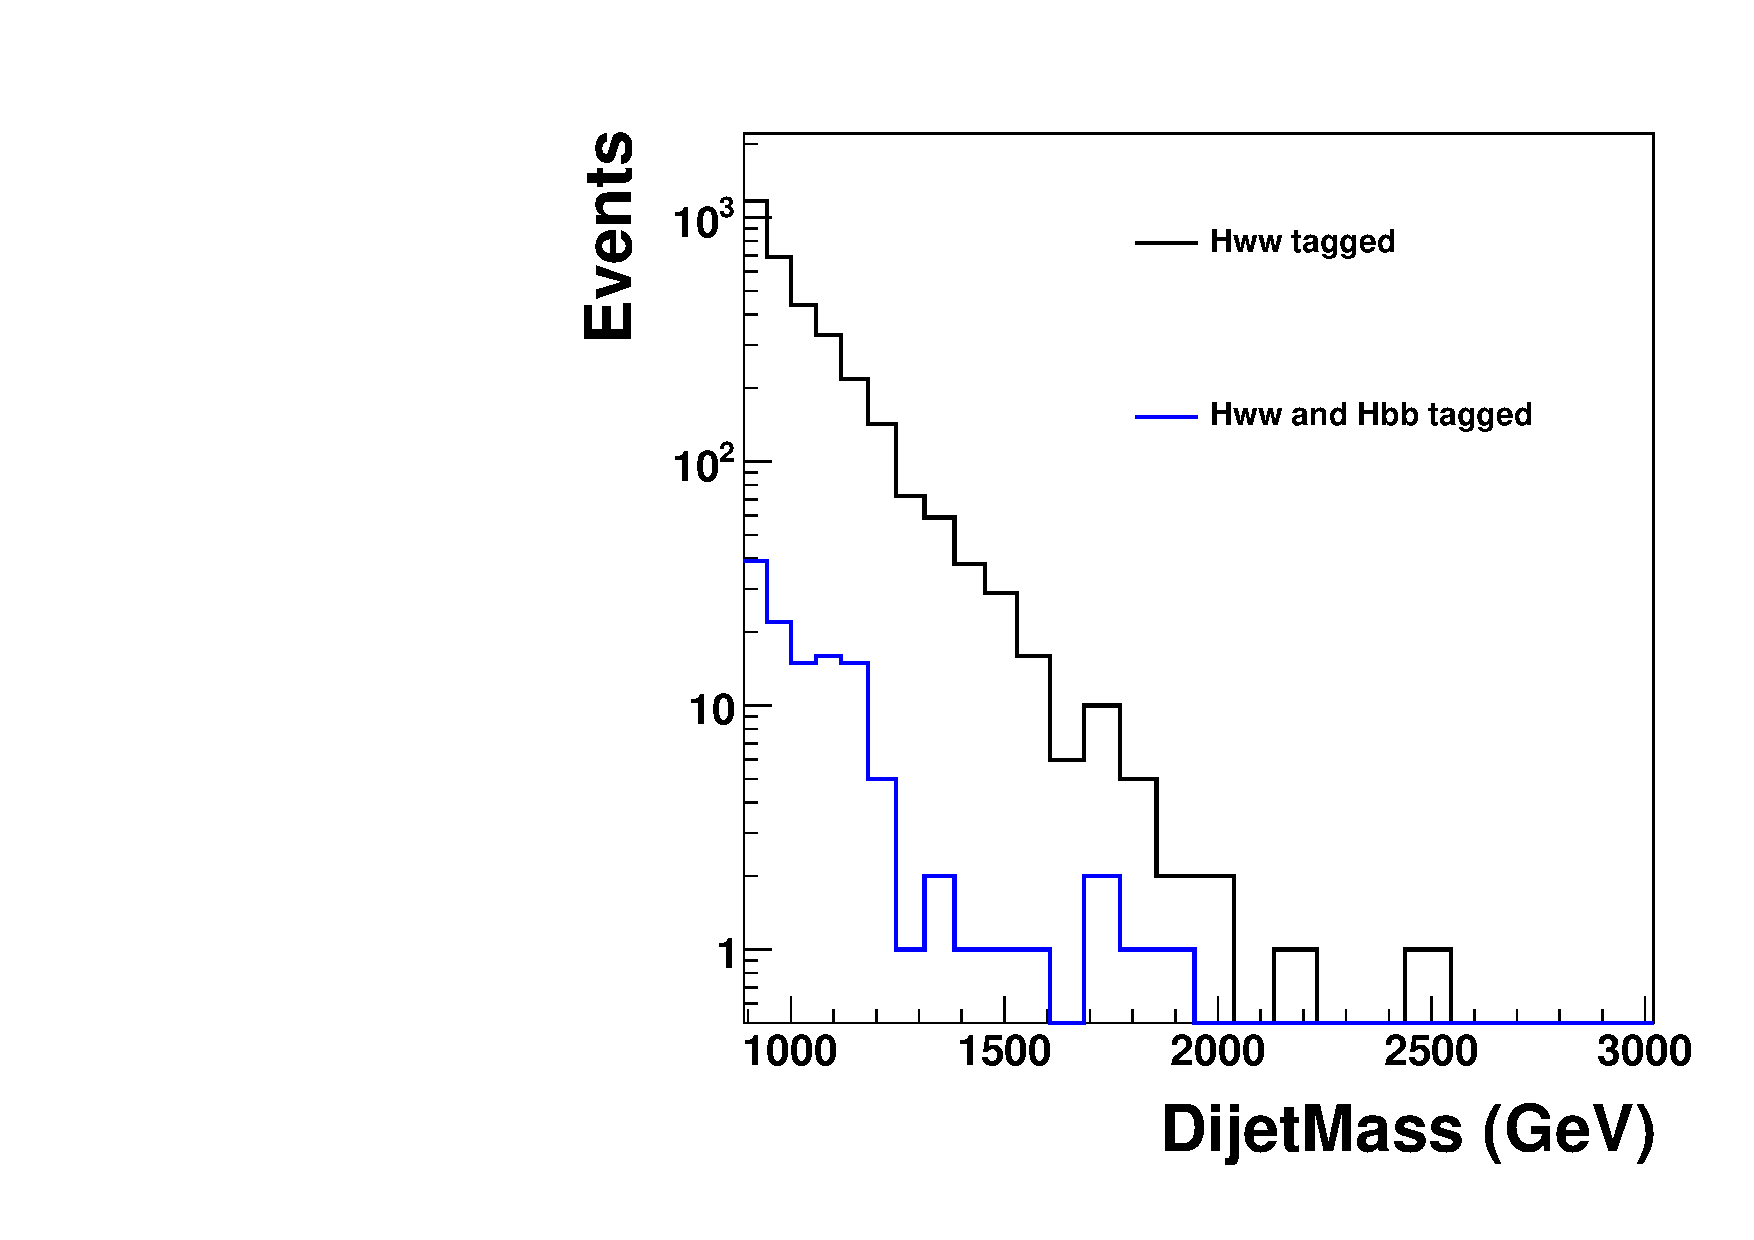
\includegraphics[width=0.49\textwidth, height=0.45\textwidth]{HqqqqZqqfigs/HbbHww/HighPurity.pdf}
%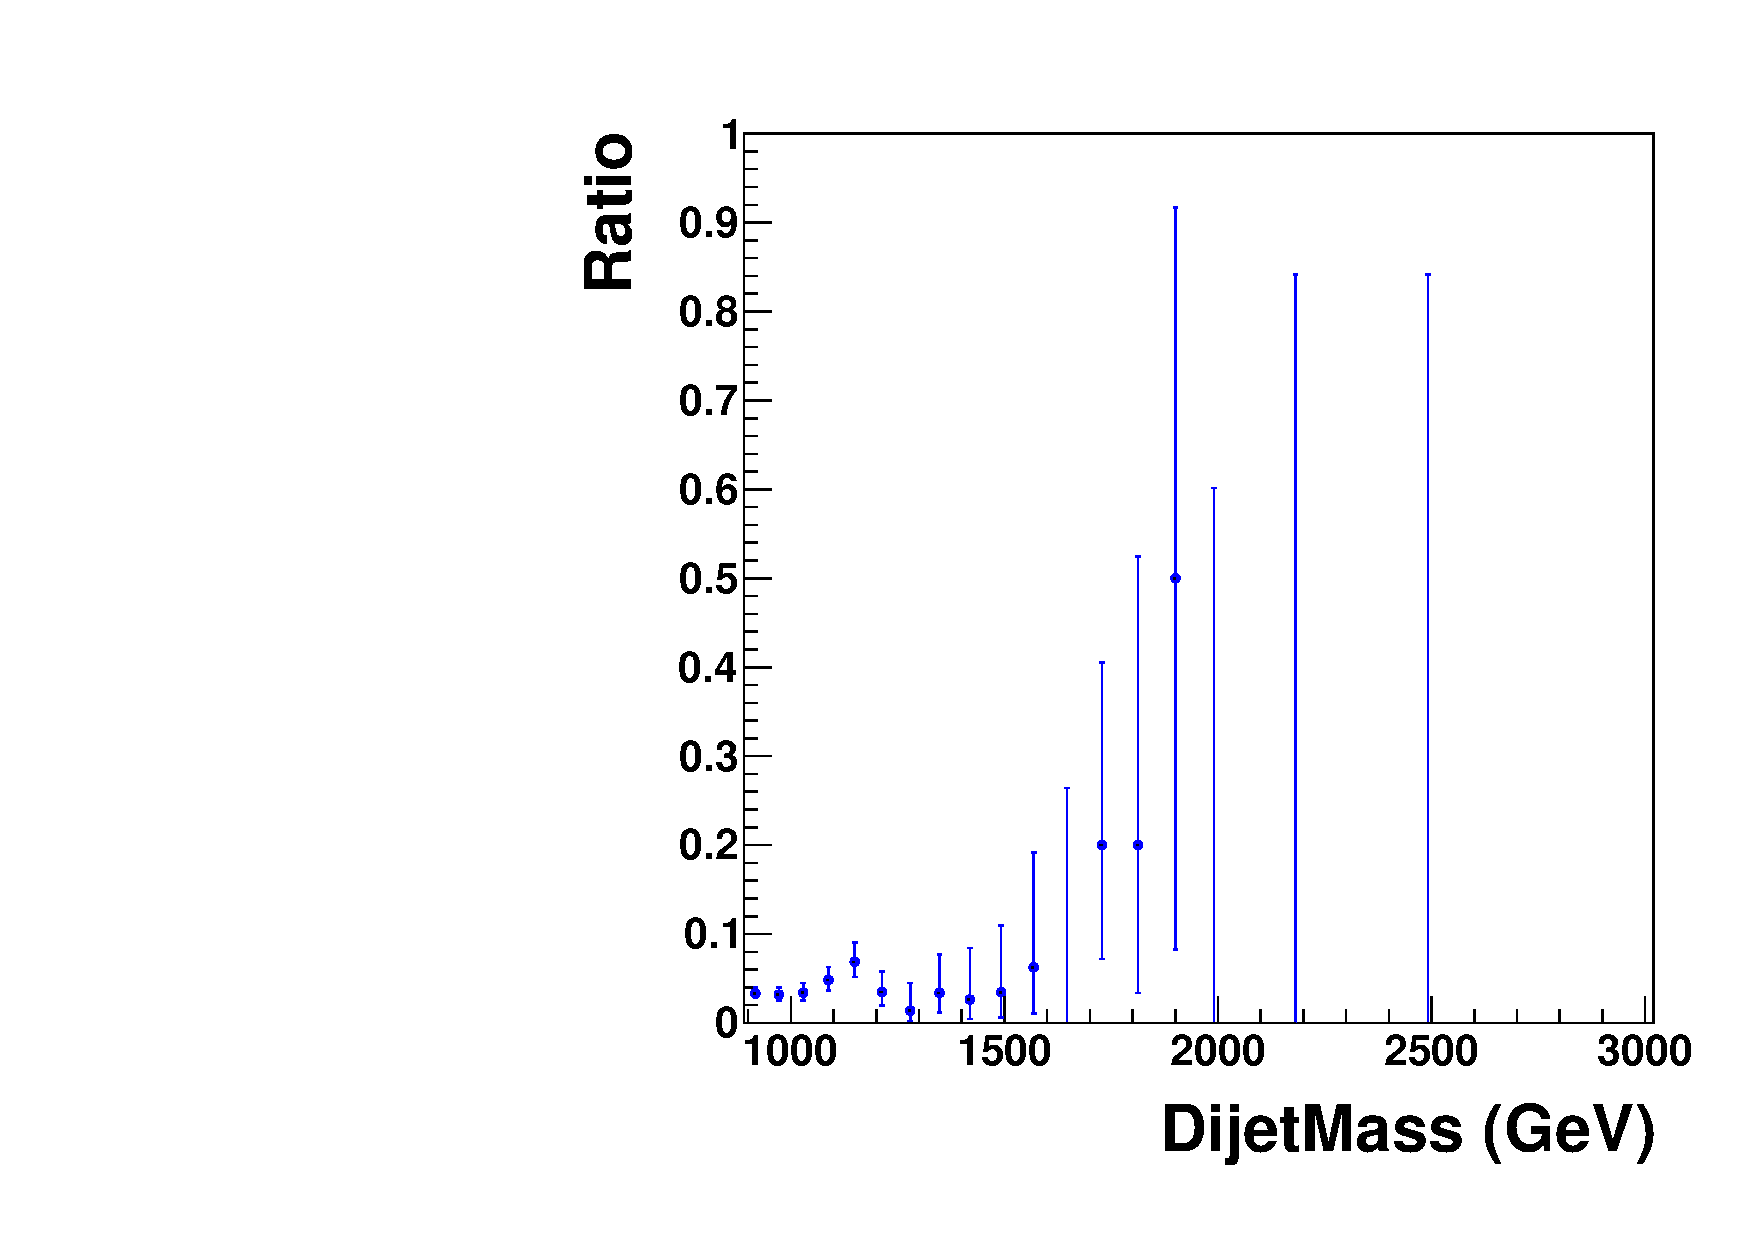
\includegraphics[width=0.49\textwidth, height=0.45\textwidth]{HqqqqZqqfigs/HbbHww/HighPurityRatio.pdf}
%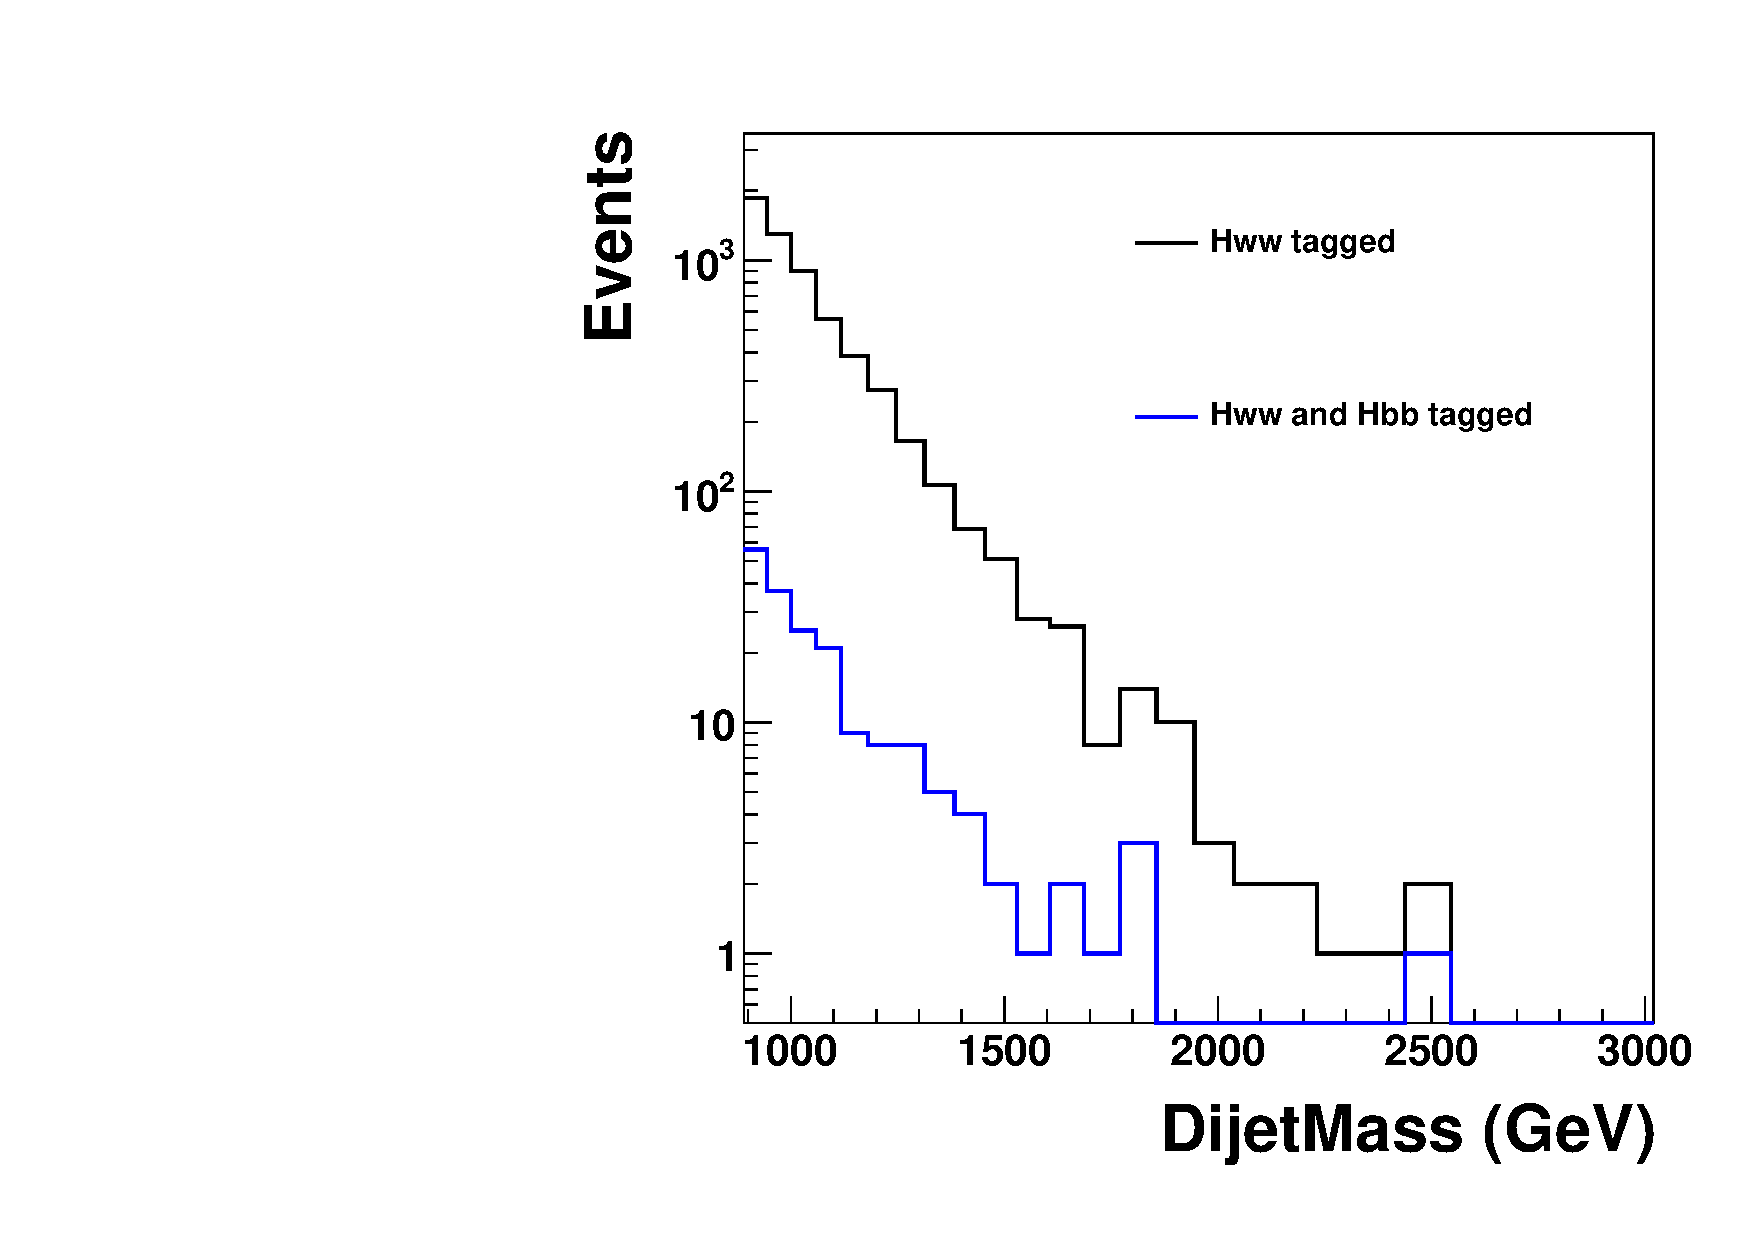
\includegraphics[width=0.49\textwidth, height=0.45\textwidth]{HqqqqZqqfigs/HbbHww/LowHPurity.pdf}
%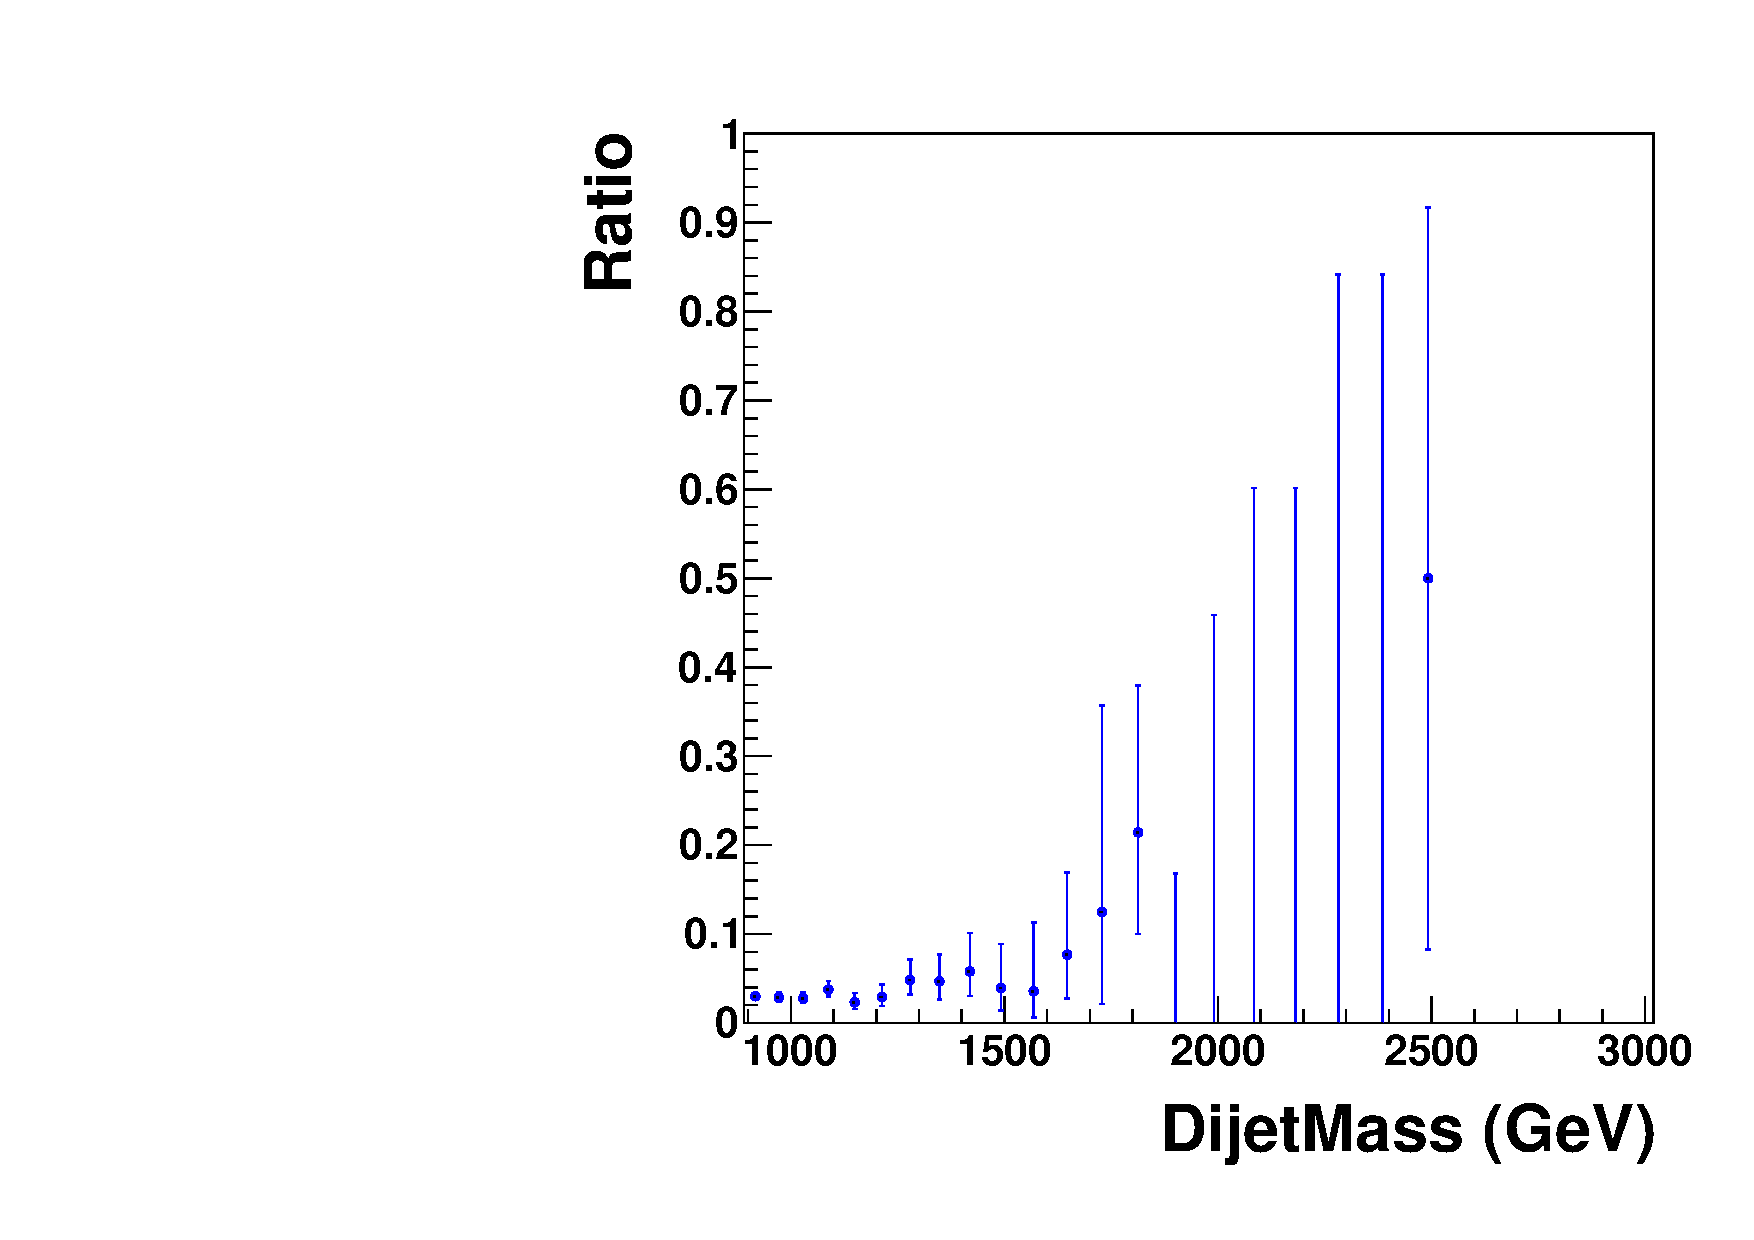
\includegraphics[width=0.49\textwidth, height=0.45\textwidth]{HqqqqZqqfigs/HbbHww/LowHPurityRatio.pdf}
%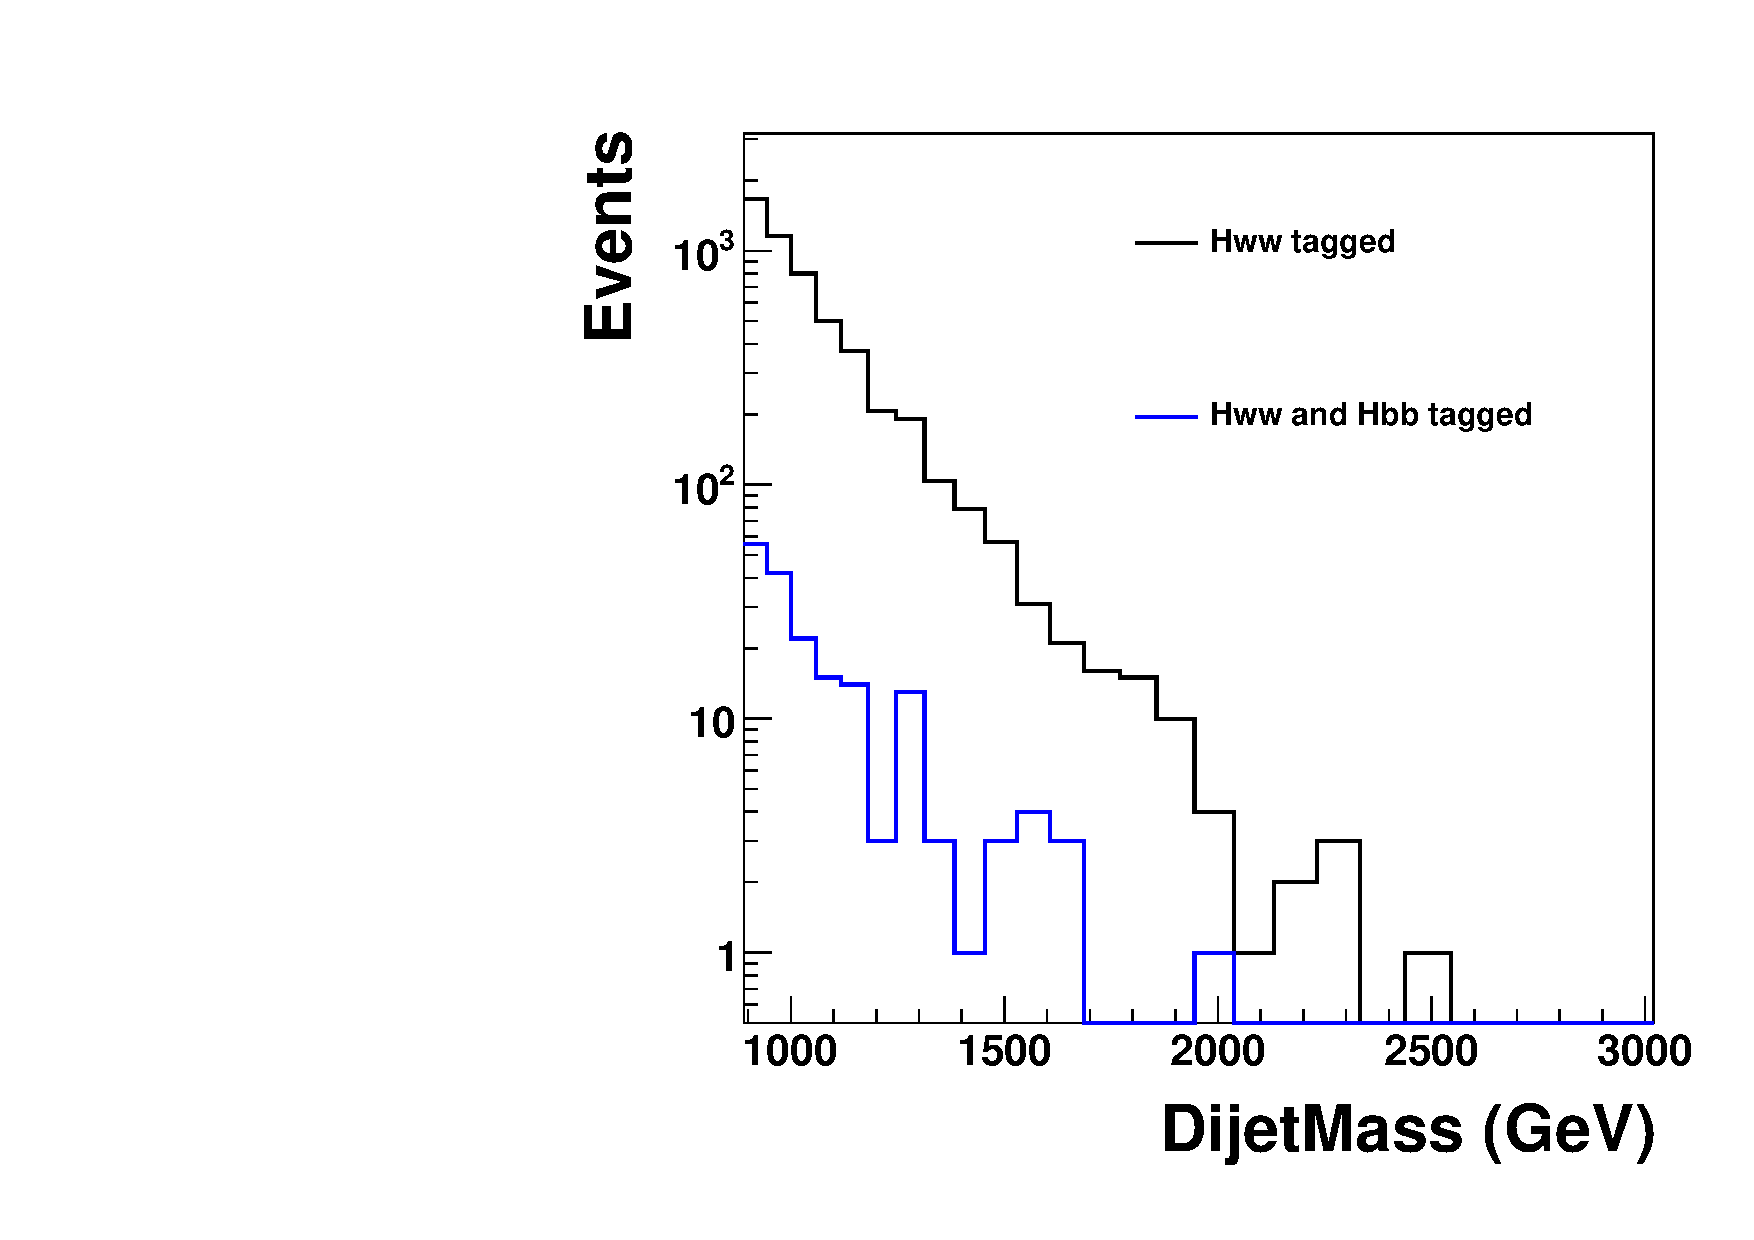
\includegraphics[width=0.49\textwidth, height=0.45\textwidth]{HqqqqZqqfigs/HbbHww/LowVPurity.pdf}
%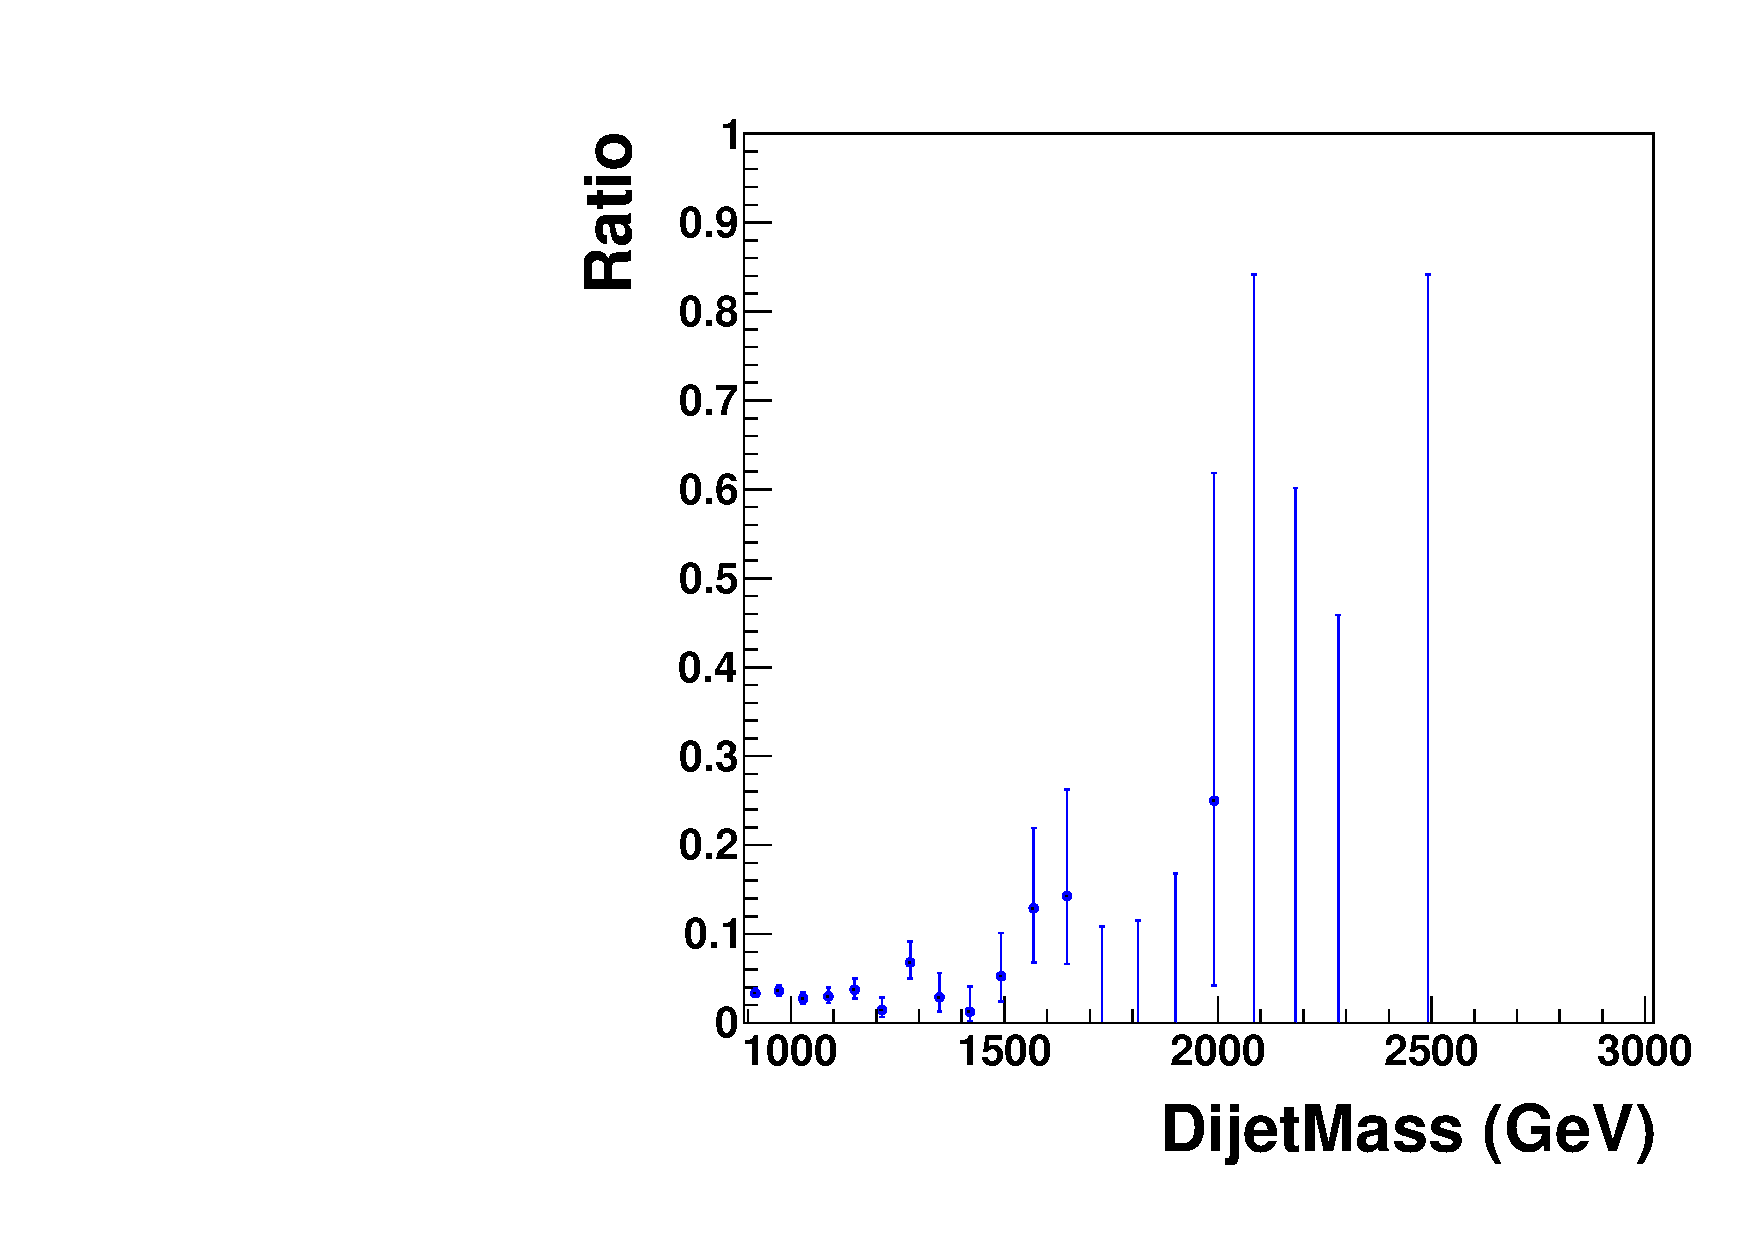
\includegraphics[width=0.49\textwidth, height=0.45\textwidth]{HqqqqZqqfigs/HbbHww/LowVPurityRatio.pdf}
%\end{center}
%\caption{ 
%  Left column: dijet mass distribution in data, for events passing the $\Hww$
%  tagger (black), and for a subset of these events passing also 
%  the $\Hbb$ tagger (blue).  Right column: the fraction of $\Hww$ tagged events
%  also tagged by $\Hbb$.  Top row: the high purity $\Hww$ tagger 
%  and high purity V-tagger.  
%  Middle row : the low purity $\Hww$ tagger, high purity V tagger. 
%  bottom row : the high purity $\Hww$ tagger, low purity V tagger. 
%}
 % Middle row: the low purity $\Hww$ 
 % tagger. Bottom: the low purity V tagger.  
%\label{fig:HbbRatio}
%\end{figure}

\clearpage
\subsection{Summary of Higgs and W/Z tagging categories}
\label{sec:total}
%Thus we arrive at the final division of events into mutually exclusive
%categories:
%\begin{itemize}
%  \item events that pass $\Hbb$ tagger.
%    \begin{itemize}
%      \item events that further pass high-purity V-tagging.
%      \item events that further pass low-purity V-tagging.
%    \end{itemize}
%  \item events that fail $\Hbb$ tagger, but pass $\Hww$ tagger.
%    \begin{itemize}
%      \item events that pass high-purity H and high-purity V-tagger.
%      \item events that pass high purity H-tagger, but low-purity V-tagger.
%      \item events that pass low purity H-tagger, but high-purity V-tagger.
%    \end{itemize}
%\end{itemize}

The W or Z jets from the signal are selected by the
V-tagger, and the Higgs candidates are selected by an OR of the two
Higgs taggers, $\Hbb$ and $\Hww$.  Both V-tagger and $\Hww$ taggers
have high-purity and
low-purity categories.  The latter are added to increase the
sensitivity of the analysis at high resonance masses, where the QCD
background is low, and a higher signal efficiency is at the premium.

We first identify the
events that pass the $\Hbb$ tagger, and only if they fail,  we
test them for the presence of the $\Hww$ tag.
Thus we arrive at the final division of events into five mutually exclusive
categories listed in Table~\ref{table:categories}.
%All the `two-dimensional' categories are shown in
%Table~\ref{table:categories}.  
For the \HwwVqq\ channel, we drop the
low-purity Higgs and low-purity V-tagging category, because it
adds only a negligible sensitivity.


\begin{table}[htb]
\begin{center}
  \caption{
        Summary of event categories and their nomenclature used in this search.
The jet mass cut is $70 < \mathrm{m_j} < 100$ GeV
for the V tag and $110 < \mathrm{m_j} < 135$ GeV for the H tag.   
    \label{table:categories}}
\begin{tabular}{ ccc}
\hline
\setlength{\tabcolsep}{24pt}
Categories                & V tag                 & H tag               \\
\hline                                                                 
\rule{0pt}{2.4ex} \HbbHP\ & $ \tau_{21} \leq 0.5$    & b tag              \\ 
\rule{0pt}{2.4ex} \HbbLP\ & $ 0.5 <\tau_{21} < 0.75$ & b tag              \\
\rule{0pt}{2.4ex} \HWWHP\  & $\tau_{21}\leq0.5$ & $\tau_{42} \leq 0.55$ \\
\rule{0pt}{2.4ex} \HWWLPV\ & $0.5<\tau_{21}< 0.75$ & $\tau_{42} \leq 0.55$ \\
\rule{0pt}{2.4ex} \HWWLPH\ & $\tau_{21}\leq 0.5$ & $0.55 < \tau_{42} < 0.65$ \\
\hline
\end{tabular}
\end{center}
\end{table}



The events from the \HbbVqq\ signals could contribute to all the five
categories, due to its large branching ratio.
The \HwwVqq\ signal events contribute only in events that fail
$\Hbb$ but pass $\Hww$ tagger; their contribution to
$\Hbb$ tagged sample is negligible.
The contributions from other Higgs decay modes to all these five categories
is tiny compared to \HbbVqq\ and \HwwVqq\ yields.  
We will not specifically study them, but include them as
 systematic uncertainties.
% due to their contribution.



\subsection{Signal acceptance and efficiencies}


To enable the results  
to be applied to other models of similar final states, 
we utilize simulations to derive the geometrical acceptances
and the selection efficiencies, presented separately in 
Figures~\ref{fig:acceptance},~\ref{fig:HbbZqqOverallEff}, and~\ref{fig:HwwEffAll}.
%To enable reinterpretation of
%the results in models with different acceptances, 
%in the following 
The global efficiency is 
approximated by the product of acceptances and 
the W/Z and H tagging efficiency, restricted
to final states where the W/Z and H bosons decay 
hadronically. A matching 
of the generated
W, Z, and H bosons, and their
reconstructed single jets
is required within
$\Delta R = \sqrt{(\Delta\eta)^2 + (\Delta\phi)^2} < 0.5$ 
as a part of the acceptances. 
The products of acceptances and the W/Z and H tagging efficiency, 
ignoring leptonic decays and the correlations between
detector acceptance and W/Z or H tagging, 
agree to better than 10\% with the full event simulation.
In the interpretations reported in this search,
the global efficiency is estimated from the full simulation
of signal events, without applying the matching requirement.
In this way, the correlations
between the acceptance and W/Z and H tagging efficiency 
are properly taken into account.
However, when interpreting this search in terms of 
W/Z and H tagging efficiency for an arbitrary model 
an additional uncertainty of 10\% should be folded in. 

The acceptance, shown in Fig.~\ref{fig:acceptance} 
as a function of the dijet resonance mass for several
signals, takes into account the angular 
acceptance ($|\eta| < 2.5$, $|\Delta\eta|<1.3$)
and the matching of the W, Z, and H 
bosons with their reconstructed single jets.


The expected tag probabilities of the \PW, Z, and H selection 
criteria for
signal and data events in different event categories are shown
in Figs.~\ref{fig:HbbZqqOverallEff} and~\ref{fig:HwwEffAll},
 as a function of $m_\mathrm{jj}$. 
The $\PW/\cPZ$ and $\Hww$ tagging efficiencies 
for signal events in the HP categories
drop at high \pt, %while they are more stable in the LP categories,
primarily because the $\tau_{21}$ and $\tau_{42}$ 
 distributions are \pt-dependent.



The MC modelling of V-tag efficiency is validated 
using high-\pt~${\rm W \to q' \bar{q}}$
decays selected from a data sample enriched 
in semileptonic ${\rm t\bar{t}}$ events~\cite{JME-13-006}. 
Scale factors of $0.86 \pm 0.07$~and
$1.39 \pm 0.75$ are 
applied to the MC events in the HP and LP V tag categories, 
respectively, 
to match the tagging efficiencies
 in the top pair data. 
The decay of $\Hww$ produces a hard W jet accompanied by two soft jets
from the off-shell W boson.  
As the $\Hww$ tagger is also based 
on the $N$-subjettiness variables, 
and the measured ratio $\tau_{42}/\tau_{21}$ 
is well modelled by QCD simulation, it 
is reasonable to assume that the mismodelling 
of the shower by \PYTHIA~is similar to that 
in the case of V tagging.
The $\Hww$ tagging efficiency scale factors are extrapolated
using the same technique as 
for V tagging for both the HP and LP categories, respectively, with 
additional systematic uncertainties, which are discussed in Section~\ref{sec:systematics2}.
The resolution for the $m_\mathrm{jj}$ reconstruction is 
in the range $5 - 10\% $ for all the five categories.

\begin{figure}[th!b]
\begin{center}
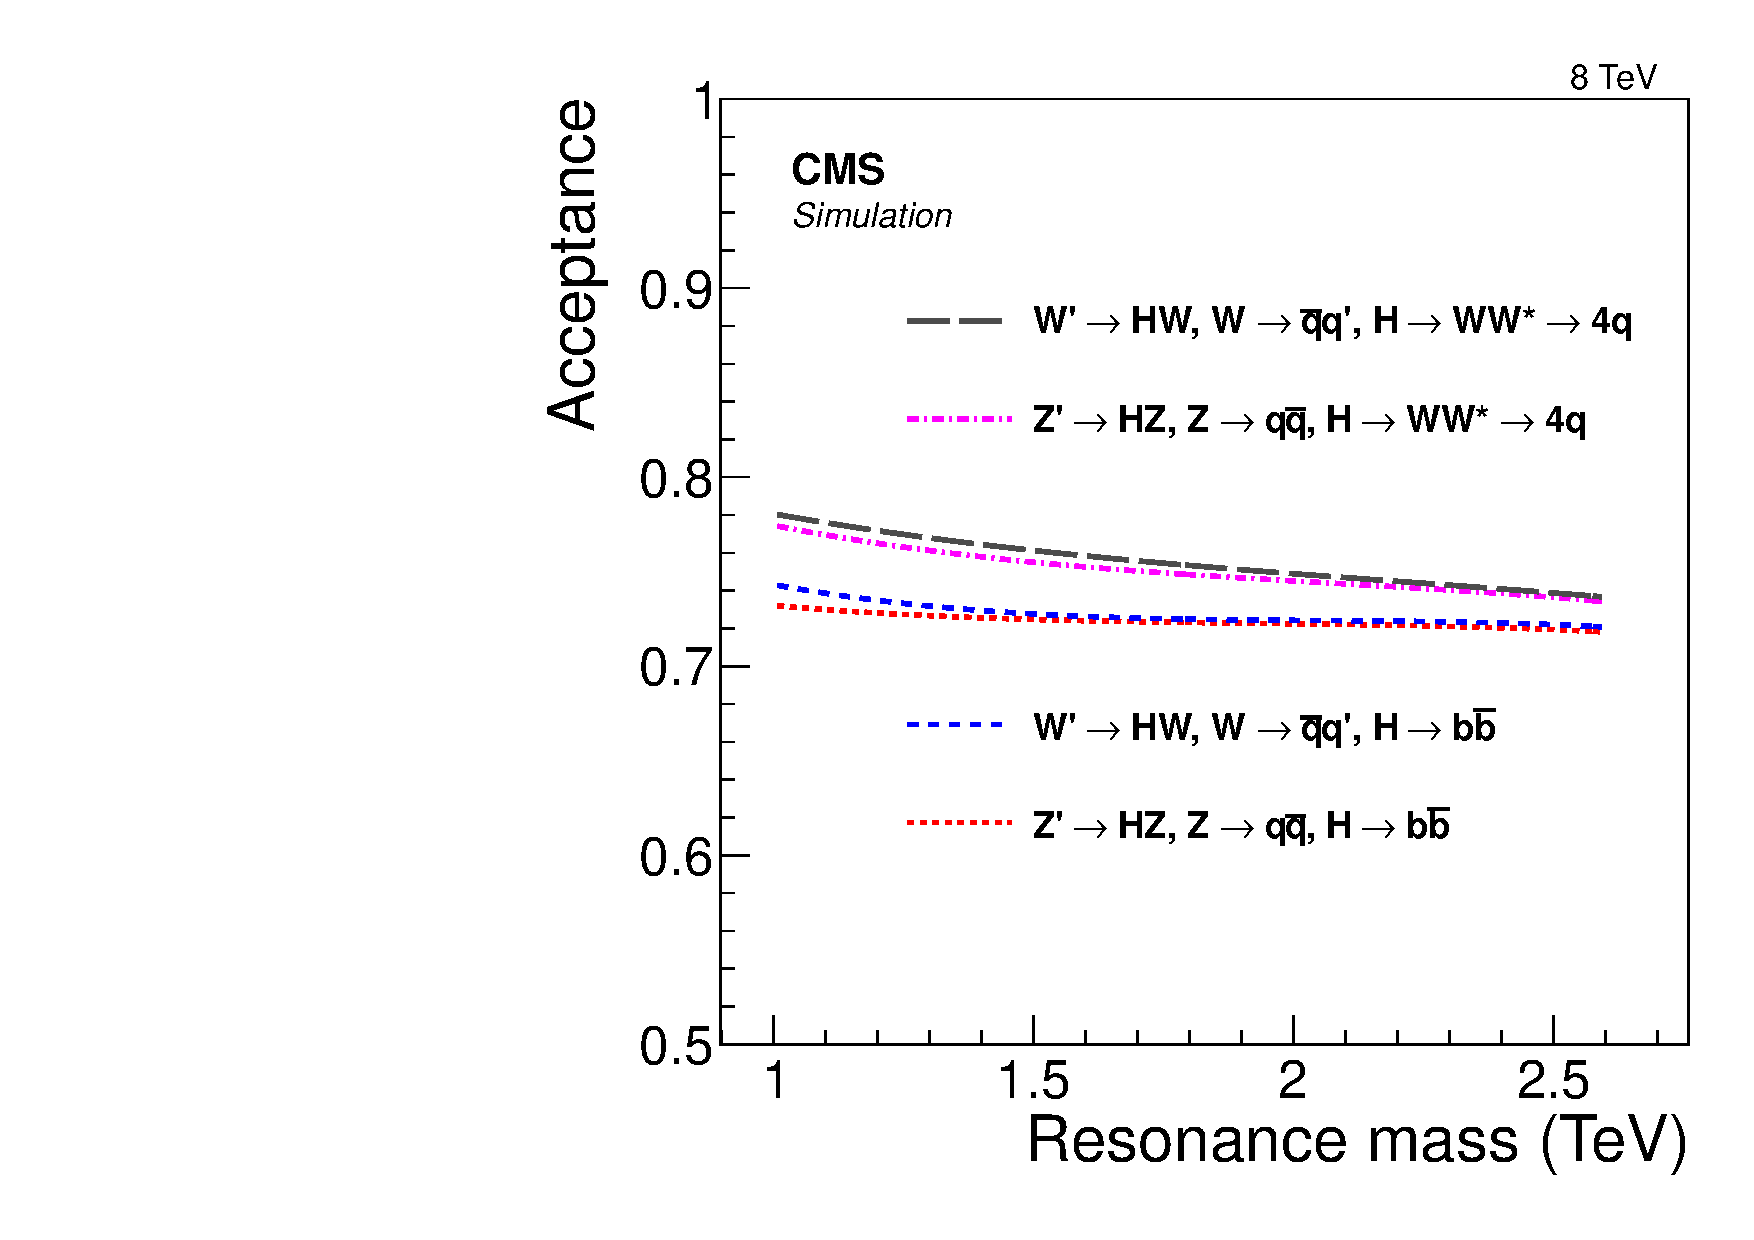
\includegraphics[width=0.69\textwidth]{EXO-14-009/figs/HbbHwwV-signal-acc-8TeV.pdf}
\end{center}
\caption{The fraction of simulated signal events for hadronically
  decaying W/Z and H
  bosons, reconstructed as two jets, that
  pass the geometrical acceptance criteria ($|\eta| < 2.5$,
  $|\Delta\eta|<1.3$), shown as a function of the resonance 
  mass.}
\label{fig:acceptance}
\end{figure}


\begin{figure}[ht!b]
\begin{center}
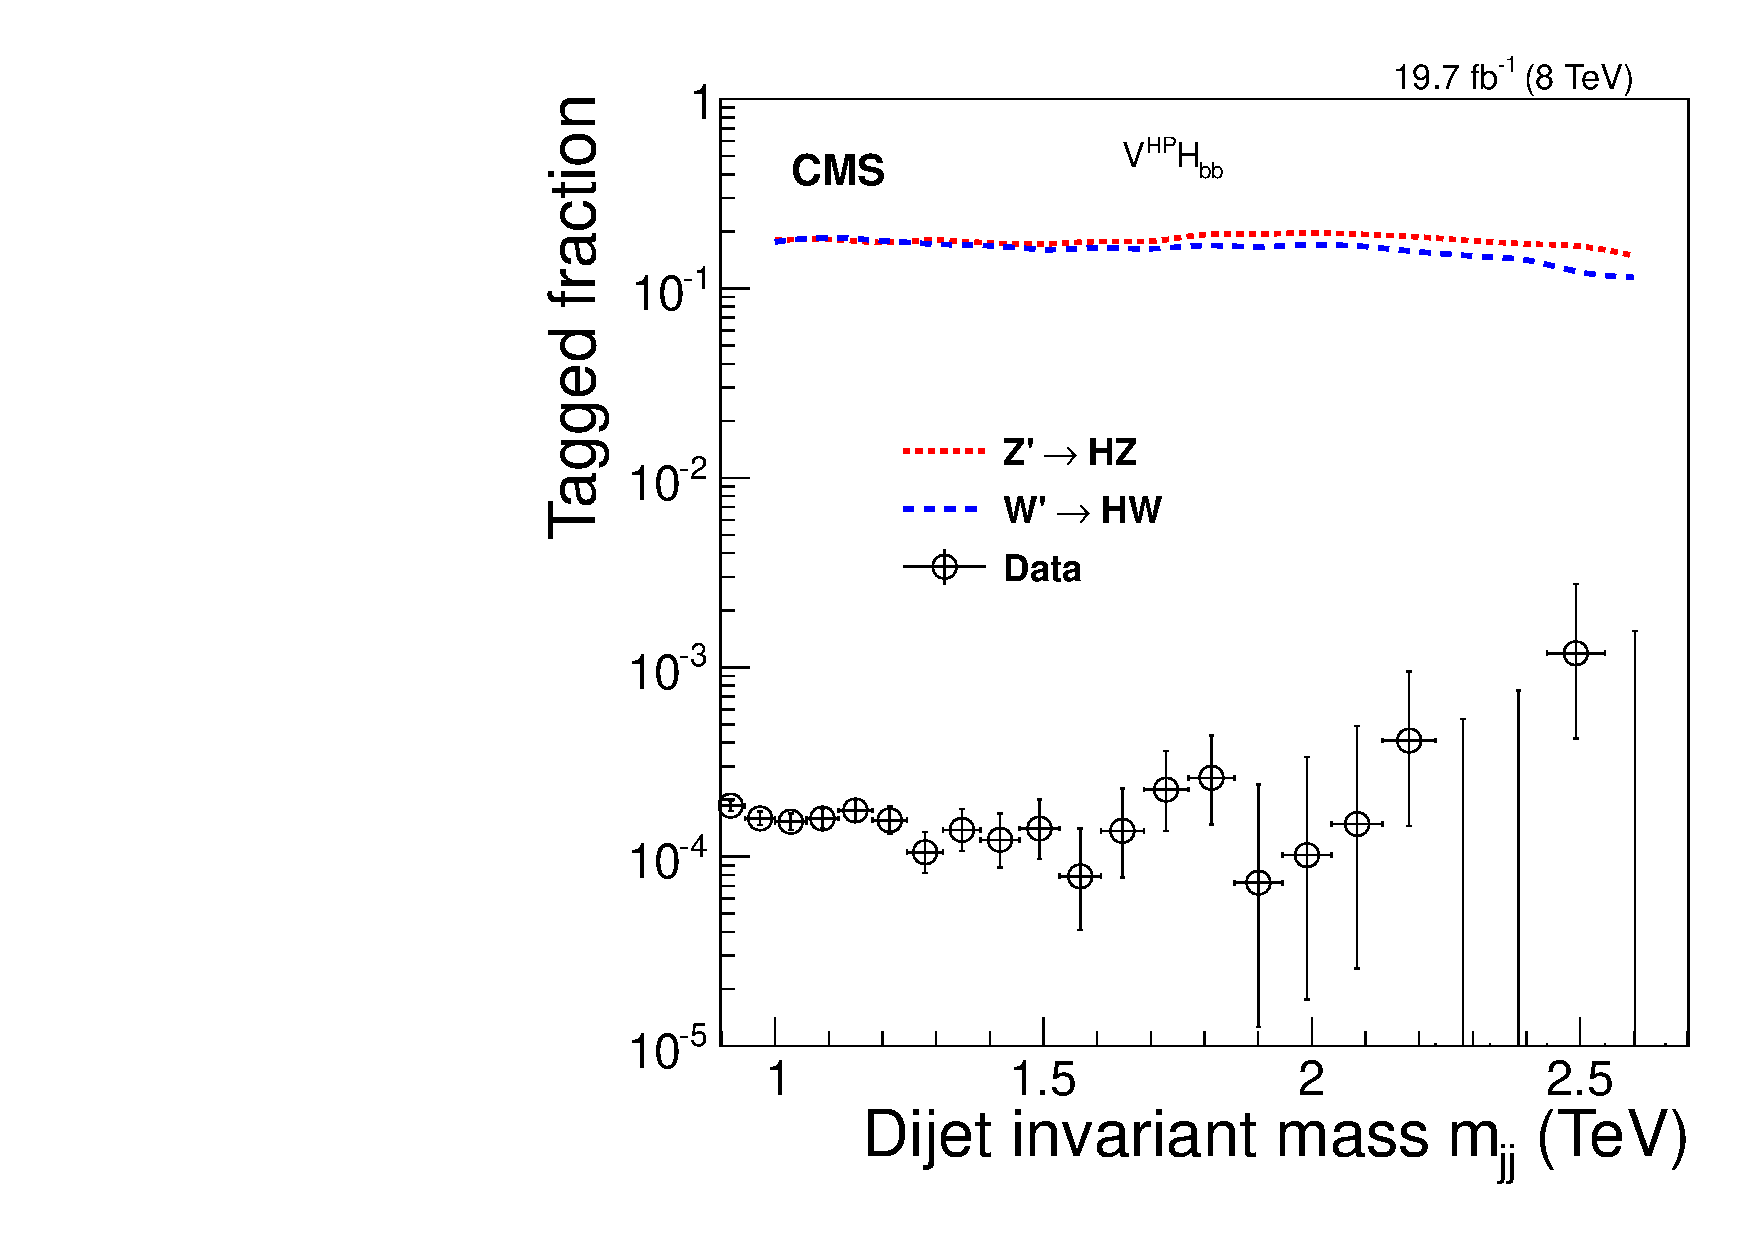
\includegraphics[width=0.49\textwidth]{EXO-14-009/HbbZqqfigs/Signal/HbbVqq-signal-taggingEff-8TeV.pdf}
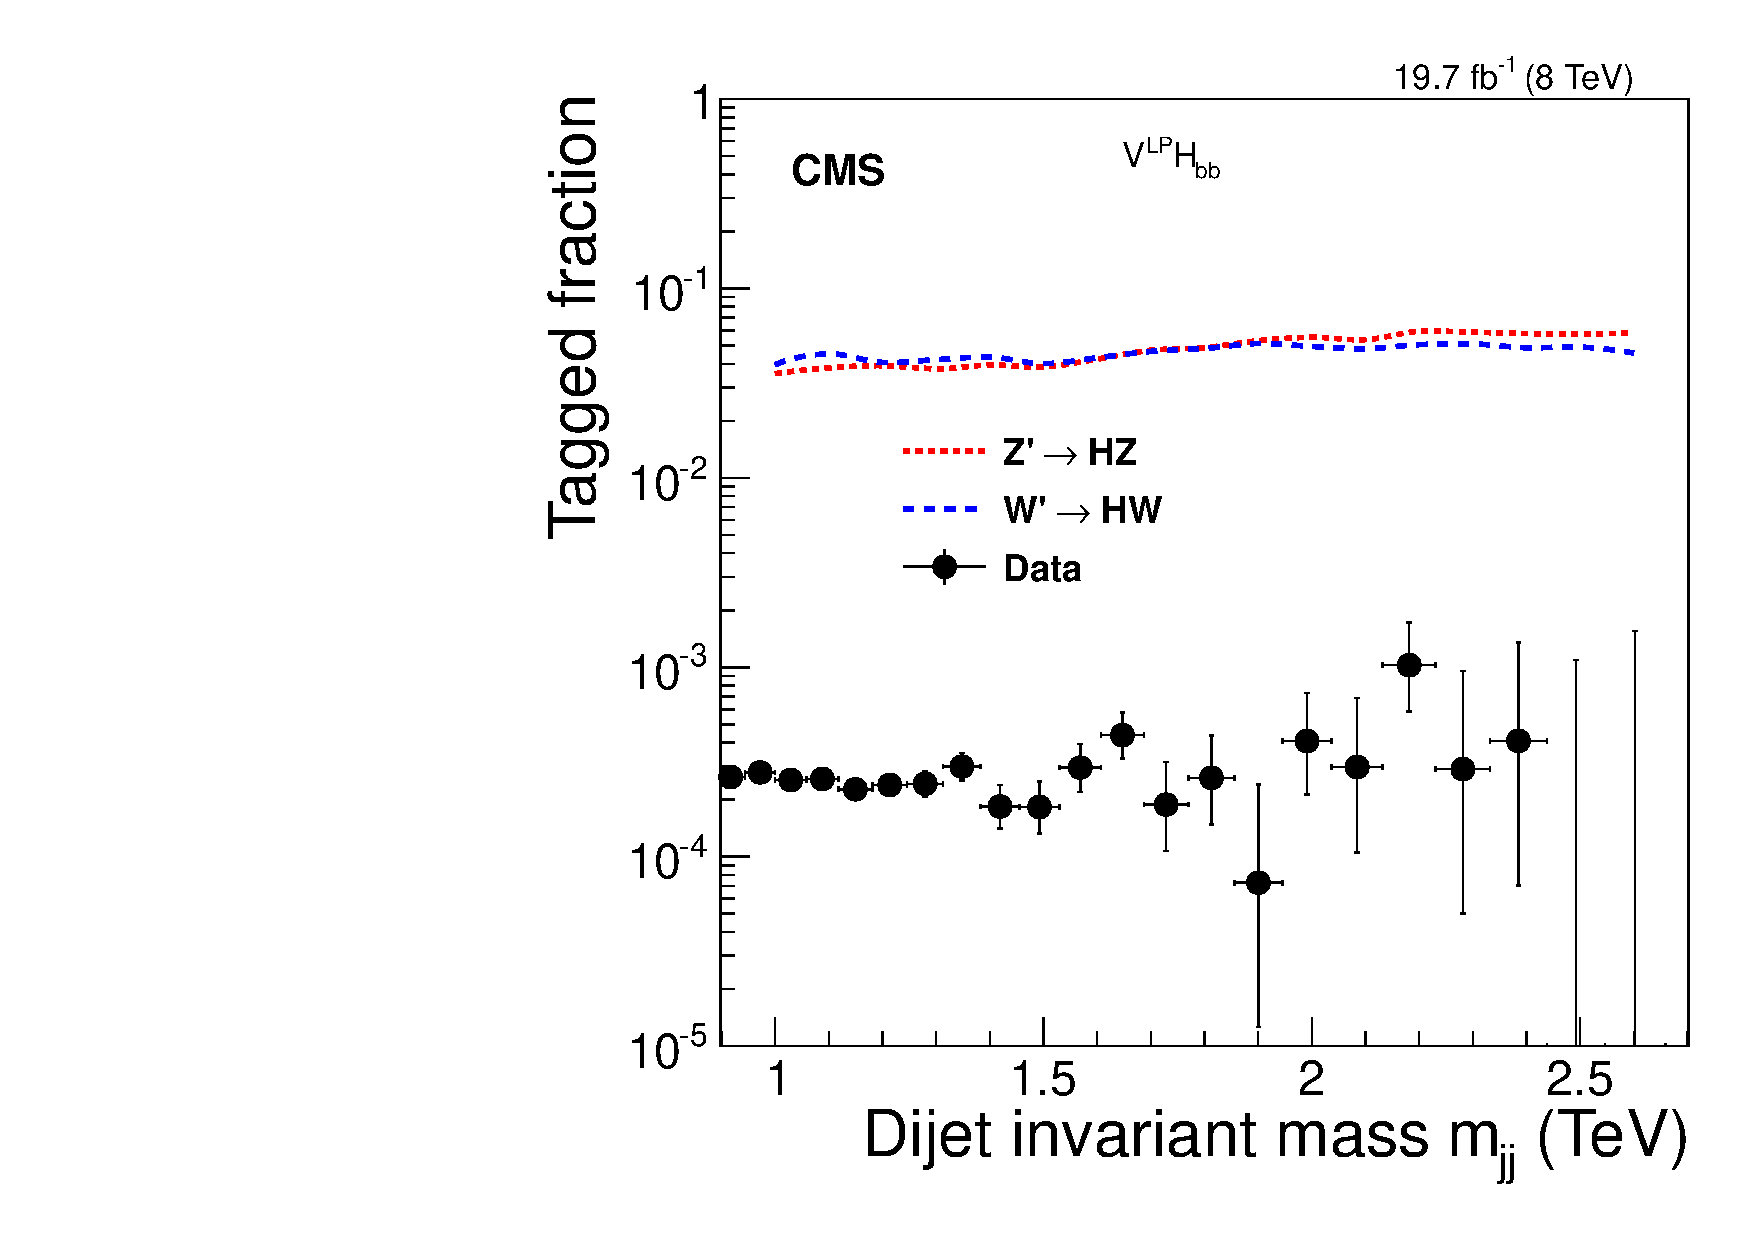
\includegraphics[width=0.49\textwidth]{EXO-14-009/HbbZqqfigs/Signal/HbbVqq-signal-taggingEff-LowV-8TeV.pdf}
\end{center}
\caption{
Tagged fractions in \HbbVqq\ signal channels and data
as a function of dijet invariant mass, for categories of 
\HbbHP\ (left) and \HbbLP\ (right). Horizontal bars 
through the data points indicate the bin width. 
}
\label{fig:HbbZqqOverallEff}
\end{figure}

\begin{figure}[!htb]
\begin{center}
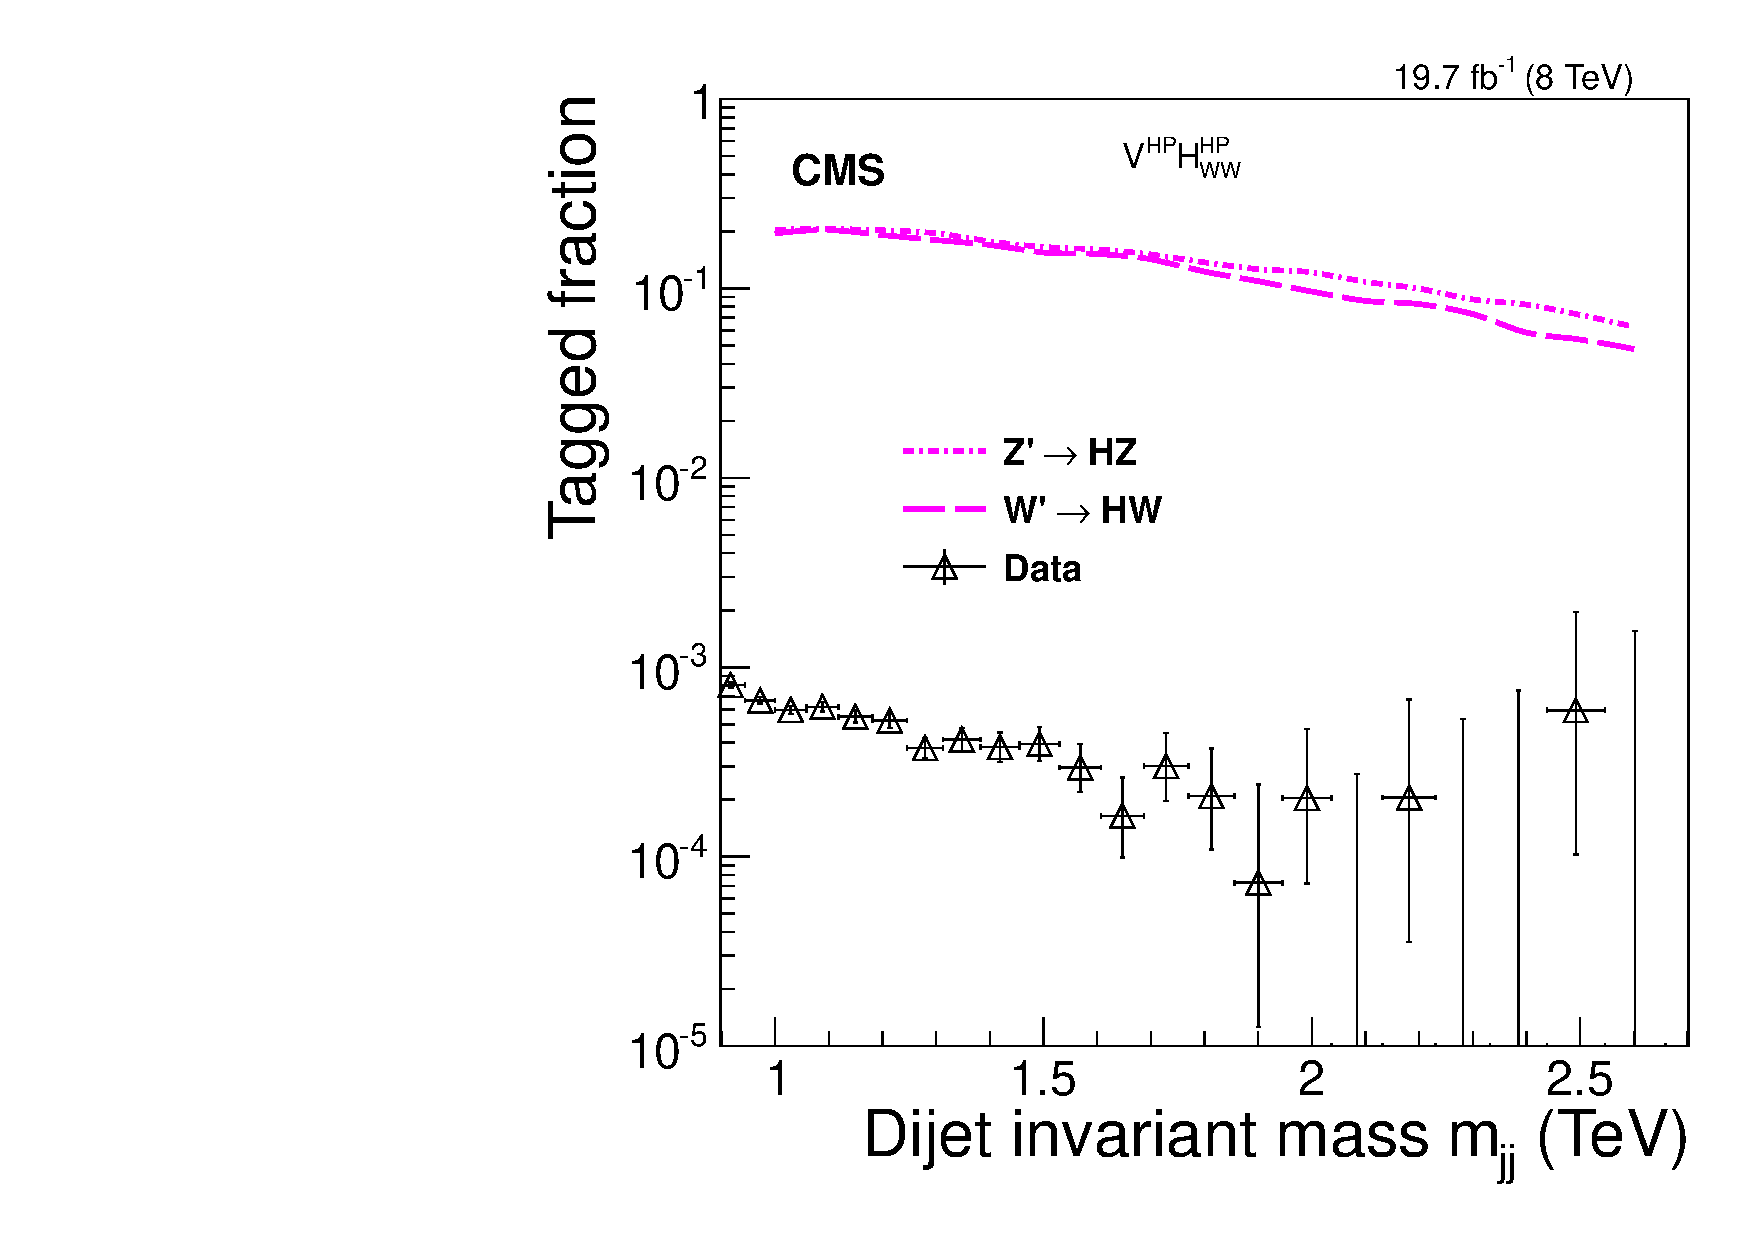
\includegraphics[width=0.51\textwidth]{EXO-14-009/HqqqqZqqfigs/Signal/HwwVqq-signal-taggingEff-8TeV.pdf}
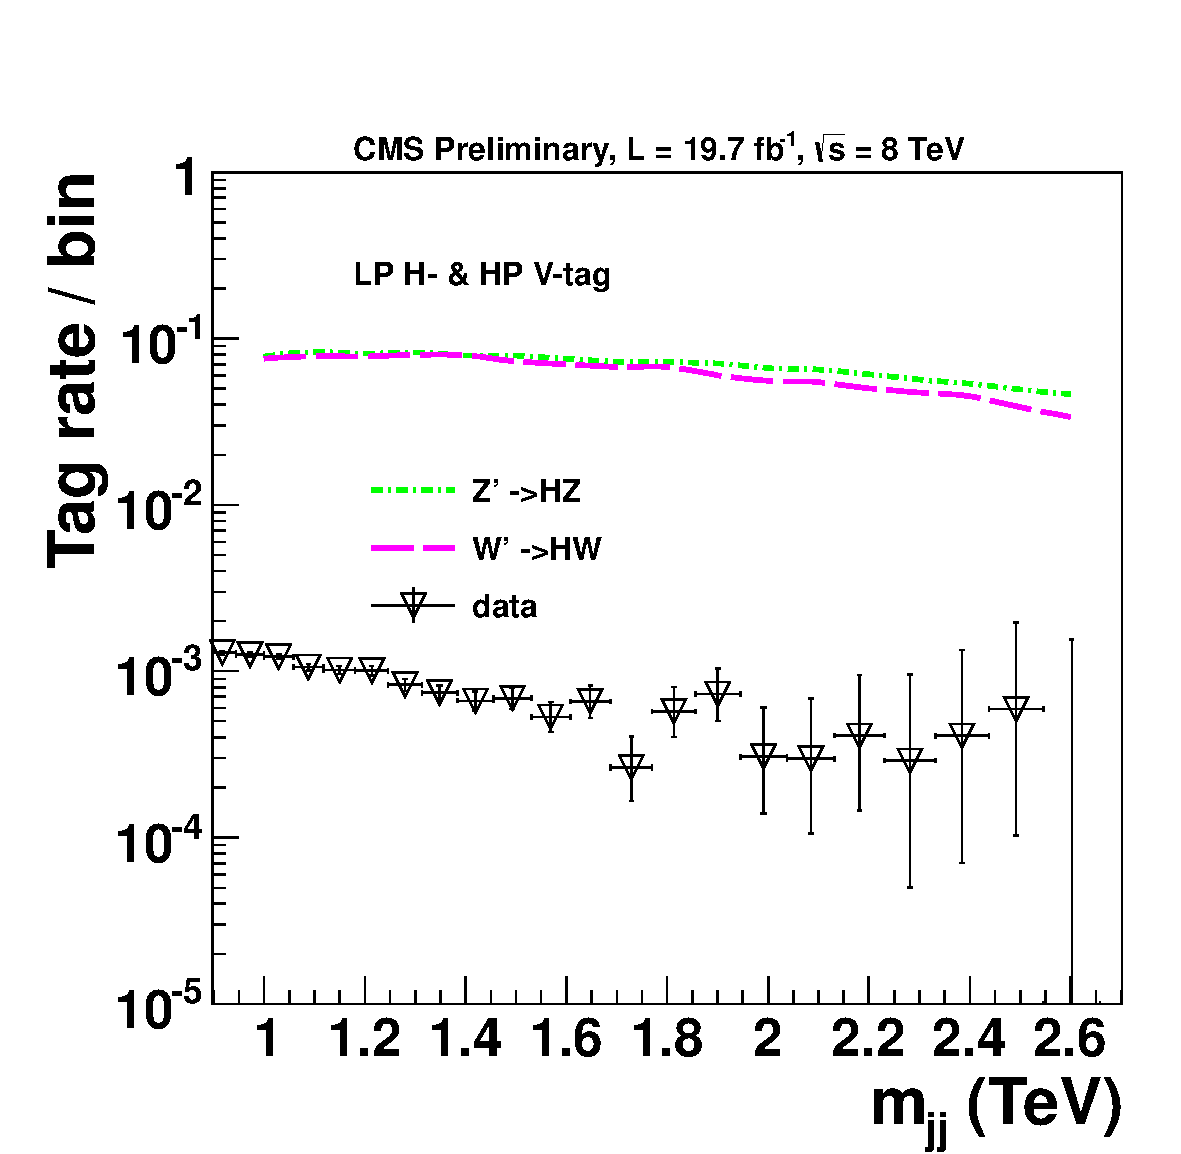
\includegraphics[width=0.49\textwidth]{EXO-14-009/HqqqqZqqfigs/Signal/HwwVqq-signal-taggingEff-LowH-8TeV.pdf}
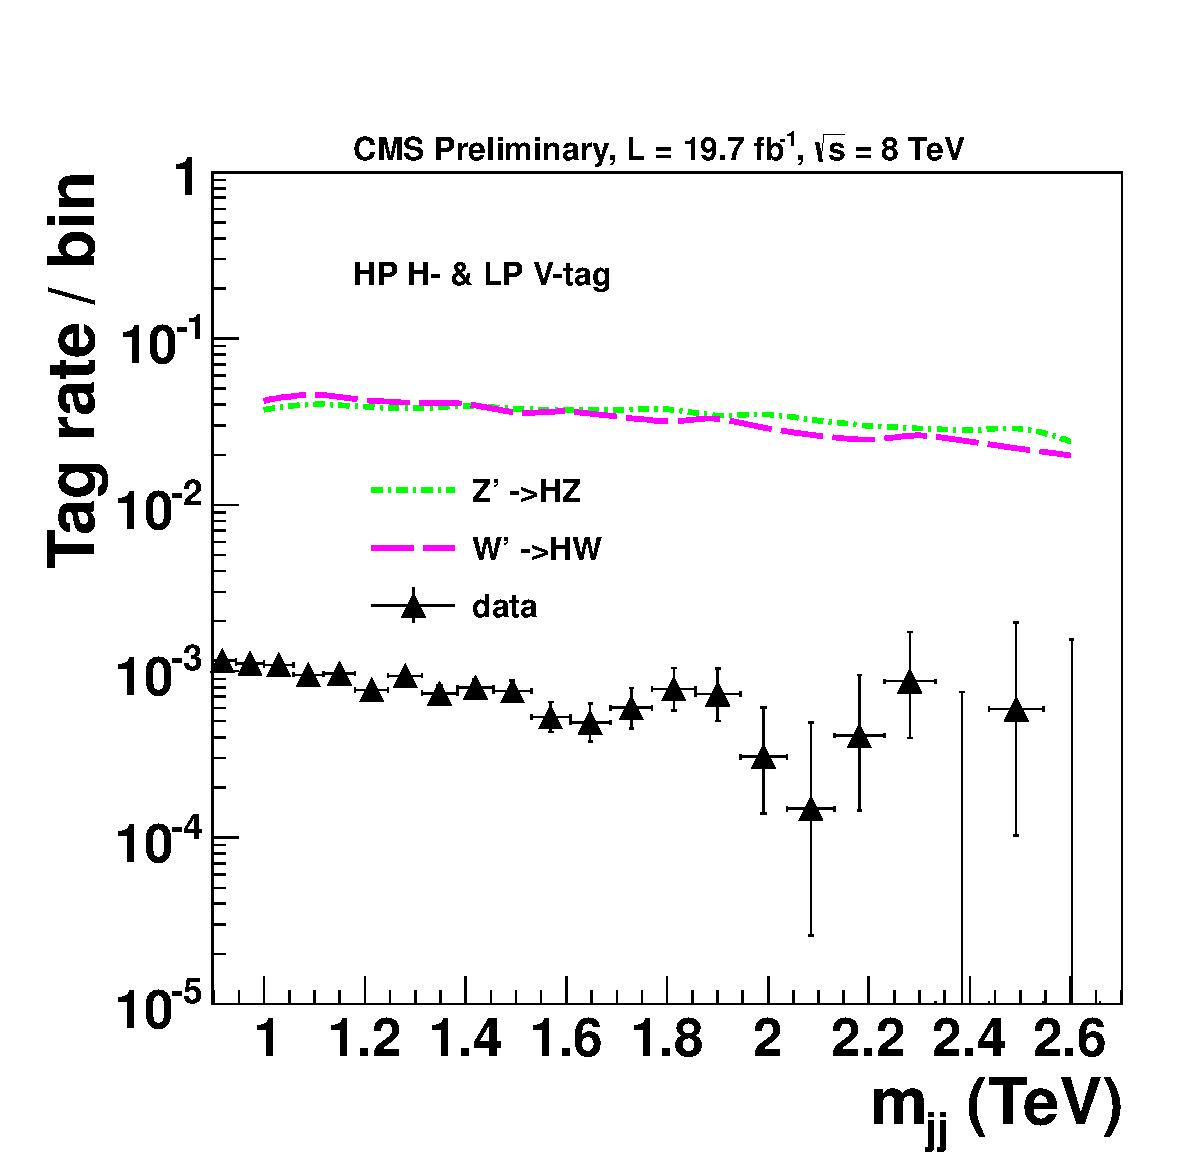
\includegraphics[width=0.49\textwidth]{EXO-14-009/HqqqqZqqfigs/Signal/HwwVqq-signal-taggingEff-LowV-8TeV.pdf}
\end{center}
\caption{
Tagged fractions in \HwwVqq\ signal channels and data as 
a function of dijet invariant mass, for categories of 
\HWWHP\ (top), \HWWLPH\ (bottom left) and \HWWLPV\ (bottom right). 
Horizontal bars
through the data points indicate the bin width. 
}
\label{fig:HwwEffAll}
\end{figure}


\clearpage

